\documentclass[a4paper]{article}

\usepackage[english]{babel}
\usepackage[utf8]{inputenc}
\usepackage{amsmath}
\usepackage{graphicx}
\DeclareGraphicsExtensions{.png}

\title{The Lost Vaults: Uneasy Alliance\\\small{An online multi-user Dungeon Client and Server.}\\\small{Project Proposal for group 4}}

\author{Felix Färjsjö\\(19911225-4678) \and Jimmy Holm\\(19870928-0138) \and Fredrik Larsson\\(19890422-0590) \and Anna Nilsson\\(19910804-0628) \and Philip Åkerfeldt\\(19920508-1335)}

\date{\today\\Version 2.0}

\begin{document}
\maketitle
\newpage
\begin{abstract}
A proposal for implementing a concurrent server model as the basis for an online, multi-user dungeon role playing game in Scala.
\end{abstract}

\tableofcontents
\listoffigures
\newpage
\section{Introduction}
Concurrency is becoming a more and more important facet of software development as computers rely more heavily on parallel processing and because of this the way we write programs has to change. 
This new kind of architecture brings with it a new type of problems and without adapting we will not be able to make use of the increase in processing power. 
As a way for us to explore these challenges and their solutions, we opted to work on a server-client system over a TCP/IP network connection. The problem we attempt to solve is maintaining a responsive 
environment for multiple, simultaneous connections as well as multiple active and independent sections of program logic. We represent this problem through a multi-user dungeon or 
MUD, a form of online multiplayer game, where we aim to make sure that the server maintains stable performance regardless of the number of connected users.

We decided to call the game Lost Vaults and it is a semi-traditional MUD where users interact with other players and take on quests in parties 
of multiple players working towards a common goal while still looking out first and foremost for themselves. It is possible to adventure as a group of one person, but the focus of the 
game will be the group dynamic offered by interaction with other players. 
The game takes place in one of two locations, the city and the dungeon; the city being where the players may recoup from previous adventures, restock on supplies and 
form parties to delve down into the dungeons. The second location is the dungeon itself, a procedurally generated set of rooms populated with monsters, traps and treasures.
The dungeon is procedurally generated and instanced in such a way that each party of players has its own dungeon, uniquely generated when the party delves down into 
the magical caves underneath the city. Once inside, the party is given one or several quests they should take on while exploring.

As described in the game design portion of this document, there are two types of quests: group quests and player quests. Group quests are to everyone's benefit and player 
quests are individual quests of subterfuge. We aim to create an atmosphere where the players need to rely on each other to achieve the tougher group quests while at the same 
time remaining weary about each other as any one of them could be a traitor, looking out only for themselves and thus creating an air of an uneasy alliance as you enter the dungeon.

The final product of this project will be a fully functional and interactive multiplayer online role playing game called The Lost Vaults.

The relation between the concept of concurrency and our project is the ability to have more than one player active in the game at the same time and their interaction with each other.
\part{Design}
\section{System Architecture}
The system architecture is in this document divided into  Client-side architecture and Server-side architecture. Being written in Scala, the application runs in the Java Virtual Machine and 
as such, both client and server should be able to run on any platform supporting Java VM 1.7.
\begin{figure}[hbt]
\centering
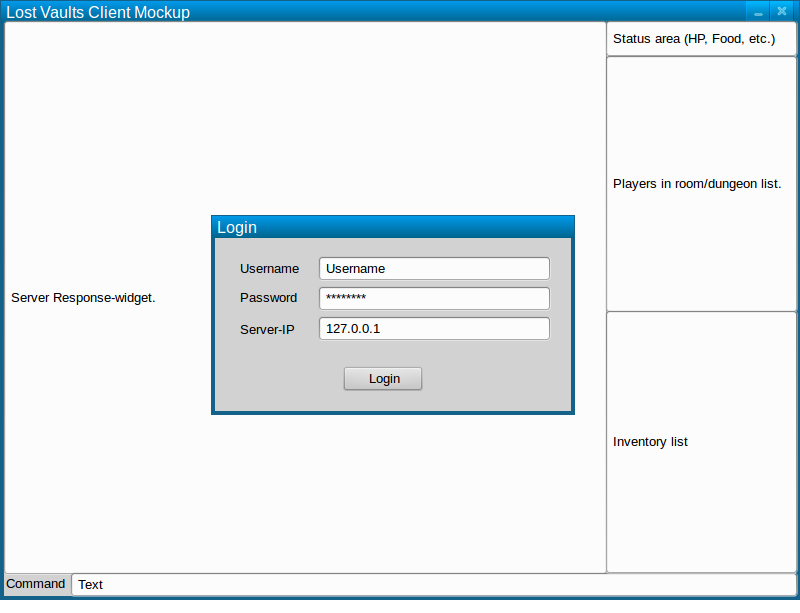
\includegraphics[width=1.0\textwidth]{clientmockup}
\caption{\label{fig:Client}User Interface mockup of the Lost Vaults Client.}
\end{figure}
\subsection{Client-side}
The design goal for the Lost Vaults client is to create something akin to a remote terminal, where no logic is performed beyond sending requests, and receiving and interpreting request responses. Ultimately, we aim to accomplish a client-side implementation that is easily extensible when the server's implementation of game logic increases, i.e. a system we can add to by simply adding new requests and responses.

As seen in Figure \ref{fig:Client} the client window is divided into several text areas displaying relevant information to the player. The main area is for regular server responses and will contain room descriptions, player chat messages, system information messages and similar.
The right side of the client is reserved for persistent information that the player may need to quickly reference. The top division contains information about the player's own character, listing the player's health and combat stats as well as the group's remaining food.

The bottom of the window contains the command input field, where the player types in commands in accordance to a strict syntax listed under the server architecture below.
Upon starting the client, the player is faced with the login window shown in the center of the mockup, where the player can enter their username and password as well as the server IP address to connect to.

The client GUI will be implemented using Java's Swing UI library and integrated into Scala to utilize Akka's TCP capabilities.
\subsubsection{Class Model}
The client is structured up into four distinct classes as described by figure \ref{fig:ClientArch}. The classes PlayGame and PlayGameCommunication work together to create a bridge between the TCP layer and the GUI, with PlayGame accepting messages from TCPClient and passing it along to the GUI through PlayGameCommunication. 
Likewise, the GUI sends data over the network  using method calls in PlayGameCommunication which passes it along to PlayGame and then TCPClient.
\begin{figure}[hbt]
\centering
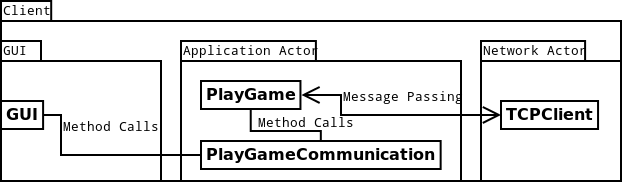
\includegraphics[width=1.0\textwidth]{clientuml1}
\caption{\label{fig:ClientArch}Client class relationship model.}
\end{figure}
\subsection{Server-side}
The server-side system architecture is further divided into the sections Concurrency model, Actor Model and Class Model. The first describes our choice of concurrency model and the 
reasoning behind it, the second describes  the function of the five major actor types of the Lost Vaults server and the final gives a more in-depth description of the 
class relationships used by the server.
\subsubsection{Concurrency Model}
We are opting to use the Actor Model for the project as we during our initial design discussion managed to isolate behaviour into several smaller and largely independent sections, 
which could with ease be made to share data only through message passing and thus avoiding the problem of deadlocks by removing shared data from the equation. 

In order to implement this kind of system with the greatest efficiency, we have chosen Scala as the language for the server as scalability is one of the fundamental design goals 
of the language. Per recommendation by the Scala language creators themselves and because of the library's strengths and ease of use, we decided to use Akka as our actor library and to make use of Akka's TCP 
library for network communication. Its simple integration also  guided our decision towards choosing Scala and Akka as the language and library of choice even for the client, as mentioned in the previous section.

\subsubsection{Actor Model}
\begin{figure}[ht]
\centering
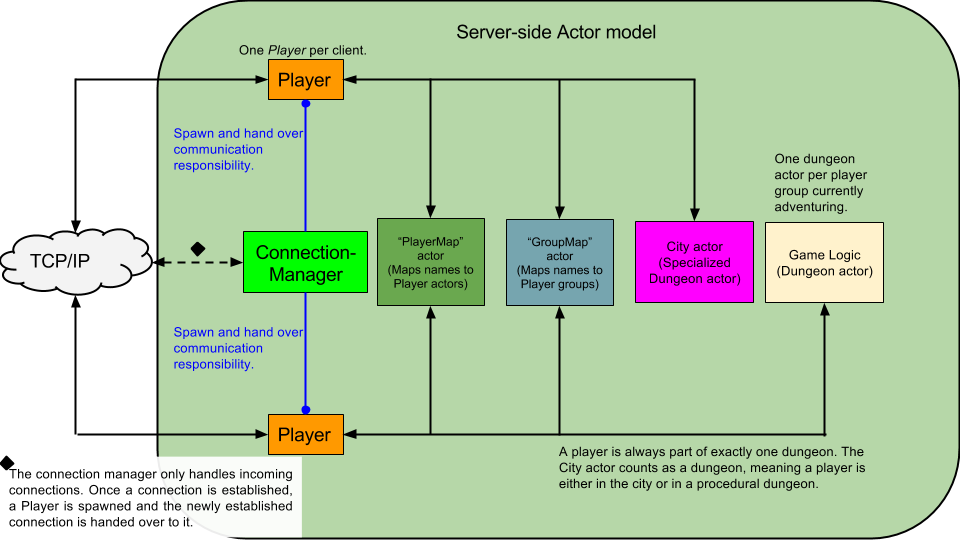
\includegraphics[width=1.0\textwidth]{serveractormodel}
\caption{\label{fig:ServerActorModel}Diagram of the server actors' interactions.}
\end{figure}
The server side is divided up into several processes using Akka's actor library to enforce the actor concurrency model in accordance with figure \ref{fig:ServerActorModel}. Only two types 
of actors communicate directly with the network through TCP/IP, the Connection Manager actor and the Player actors. The Connection Manager actor serves as the entry point for incoming
connections, and is in charge of spawning Player actors as new top-level actors before registering them as the newly established connection's listener. As the listener, the Player actor
will receive and send data over the network through the established connection. The Player actor is in charge of all things related to the clients, such as the specific player's attributes,
as well as verifying login attempts through communication with the PlayerMap and it is through the Player actors that the other actors can send messages over the network when necessary.

The PlayerMap actor and GroupMap actor serves two specific utility functions, the first of which is to map a string, the names of all connected players, to the actors controlling the player 
with that name. Through this actor, another actor can quickly and easily send messages to a specific actor based on its name - an important feature for commands acting on other players, 
such as \textit{WHISPER}. It also allows a quick and simple way for the Player actor to ensure no more than one player of a given name exists on the server at any given time.

The GroupMap actor performs a similar function as PlayerMap, however it links player names with player groups instead of player actors. A player group, as described in the game design 
section of this document, is a collection of one or more players who together can enter a dungeon that is procedurally generated for them. The purpose of this actor is to facilitate 
forming and joining other groups of players. Using the GroupMap, it is enough to join a player by name to be included into that player's group, or have a new group formed for them.

The fourth type of actor used by the Lost Vaults server is the Dungeon actor, the actor performing all game logic. There is a special case of Dungeon actor which is called the City actor. 
The City actor is a Dungeon actor that is persistent over the lifetime of the server and has special behaviour to handle the socializing aspect of chatting and forming groups as well as trading 
with NPC \footnote{Non-Playable Character} merchants. The ordinary case of the Dungeon Actor is in charge of generating and handling a procedural dungeon of multiple, interconnected rooms layed out in a two-dimensional 
grid. It is in these dungeon rooms that players will have the ability to complete quests, find treasure, etc. The Dungeon actor is in charge of coordinating all the players that are 
currently present in the dungeon, and make sure that commands such as \textit{SAY} are relayed to the relevant players. With the exception of the City actor, the Dungeon actors are 
in charge of their own lifespan after having been spawned by the City actor, and a Dungeon actor will stop itself once there are no more players within it.
\subsubsection{Class Model}
\begin{figure}[ht]
\centering
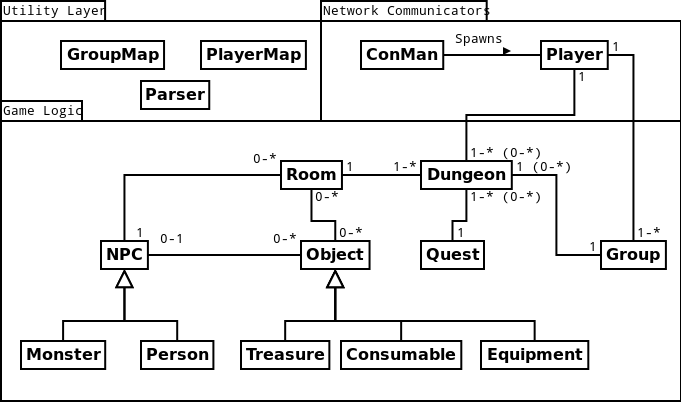
\includegraphics[width=1.0\textwidth]{serveruml1}
\caption{\label{fig:ServerUML}The server's class relationship model.}
\end{figure}
Figure \ref{fig:ServerUML} show the relationship between the different classes of the Lost Vaults server implementation and the multiplicity of relevant relationships. They are divided 
into three categories; the Utility Layer, the Network Communicators and the Game Logic. The Utility Layer provide supporting functionality to the other classes and exactly one of each 
class should exist at any given time. The Network Communicators are the ones that relate back to the network through Akka's TCP library. Of the two, ConMan, the connection manager class, 
is to be considered a singleton and only one instance should exist at any given time. The Player class however has one instance for each open connection.

The Game Logic section contains all the internal classes as well as the Dungeon class. The Dungeon class is the bridge between the Network Communicators and the Game Logic and it is 
only through a Dungeon class that a Player can perform any actions apart from the server-wide \textit{WHISPER} command. The Dungeon class keeps track of explored and unexplored rooms, 
quests, groups, objects and NPCs. The Dungeon also keeps track of all Players currently connected and associated with the given dungeon.
\section{Game Design}
\subsection{Dungeon}
The meat of the game takes place in procedurally generated dungeons, each unique to the group of players who enter that dungeon. Once a dungeon has been created and a group has 
been assigned to it, no new players may enter that dungeon. A player who dies in the dungeon will be forced to leave the dungeon, as described below, and a player who has left the dungeon 
may not reenter it.

The dungeon's room are created procedurally at the creation of the dungeon. Each cell in a two-dimensional grid is assigned a room, and random routes connecting them to a starting room are placed 
down to ensure each room is potentially reachable, provided players have enough food.
\subsubsection{Rooms}
The dungeon is made up of interconnected rooms, which may have one or more exits, each representing a door on one of the room's four walls. A room may contain any number of players, monsters 
and items. A room may also contain a ``trap'' which can be harmful as well as beneficial, performing an action on the first player to enter that room. Players may attack any other player or 
NPC occupying the same room. Combat is described in more detail below. When the combat is between players, neither player currently fighting may escape the room until one of them has fallen. 
Escaping from a battle with an NPC will cost the escaping player one extra food.
\subsubsection{Food}
Food is the main type of resource to be managed in the game as food is needed to explore the dungeon. Each player has their own supply of food, starting at a minimum of five pieces of food 
and additional food can be bought from the city merchant or be found in the dungeon. When a player enters a room that player has not yet explored, one piece of food is subtracted from their 
personal supply. Entering a room previously explored by that player does not consume food. The players' progress is therefore limited by how much food they bring with them into the dungeon.
\subsubsection{Leaving The Dungeon}
Upon leaving the dungeon, all the consumables found or brought down will be lost to the player (food and potions rot), and all treasure items that are found are sold off for gold. 
Furthermore, every player leaving a dungeon is awarded gold for the quests they have completed both as a group or individually. Dead players do not gain gold for completed quests.

If a player dies, they are forced to leave the dungeon, and gain no gold from either treasures found or quests completed.
\subsection{Player}
The player has four distinct attributes to aid her in her adventure. Life signifies the current health of the player, when life reaches zero the player dies and she will face the penalty 
described below. Defense represents her ability to withstand damage and is in direct opposite to the Attack attribute of an opposing entity. Attack then is the ability to inflict damage, 
and the damage calculation is a simple calculation of subtracting the defender's defense score from the attacker's attack score. The result, if greater than zero, is then subtracted from 
the defender's current life. If the defender's life reaches zero, she dies. The final attribute is food, and as described above it represents the player's ability to explore the dungeon 
as well as her ability to flee from combat against foes that are too dangerous. 
\subsection{Combat}
Lost Vaults uses a turn-based combat system, where each participant get their chance to attack any of the other occupants in the room. Attacking another player forces them to join in the 
combat, denying them the ability to escape the room. During player versus player combat, neither player may send a private message or perform a dungeon wide yell command, limiting their 
ability to communicate to only the room they are occupying. Combat against an NPC does not have this limitation, and players may both escape at the cost of one additional food, and they 
may use yells to call in aid from their allies.
\subsubsection{Death}
Dying in Lost Vaults carries a penalty in the form of losing all consumable items and treasures the dying player carries, as well as being forced back into the city without the possibility 
to rejoin their comrades still exploring the dungeon. This means all progress made inside the dungeon is lost upon death, as well as all gold spent preparing for the adventure. All treasure 
and consumables held by the dying player will be left on the floor of the room in which she died.
\subsection{Quests}
When entering a dungeon, the group is given one or more quests to complete which will net them extra gold upon leaving. However, individual players may also be given an additional quest, 
which they alone stand to gain from and which is in direct opposition to the group's best interest.
\subsubsection{Group Quests}
Group quests are quests that all players of the group benefit from, and completing the quest is in everyone's best interest. The reward for a completed quest is given to each player who 
is alive to leave the dungeon after completion. The group quests are as follows.
\begin{description}
\item[Kill a specified monster] The group is tasked to kill a specific monster, appropriate to the strength of the group. The monster is placed in a random location and a path is 
guaranteed from the start to the monster's room.
\item[Find an item] A specific piece of treasure is to be located and taken out of the dungeon. Similarly to the previous quest, a room is created containing the item and a path is 
guaranteed to it from the start.
\item[Kill X monsters] A specified number of monsters are to be slain. The types of monsters do not matter, and every killed monster works towards this goal.
\item[Every ally must survive] This quest works against traiterous players. Whenever a player gains the \textbf{Kill a specified player character} or \textbf{Be the only survivor} players quests, the group gains this quest.
In order for this quest to be completed, not only does everyone not tasked with a kill quest leave the dungeon but the player who does have that quest must not. That is to say, an eventual  
traitor has to bee rooted out of the group and killed in order for the group to accomplish this quest. This quest does not require a traitor be present, but if a traitor is present this 
quest will always accompany it.
\end{description}
\subsubsection{Player Quests}
Player quests are quests given to individual players and they alone stand to gain from it. It is in opposition to the best interest of the rest of the group and their rewards are 
greater than the others, providing an incentive to complete them. The player quests are as follows.
\begin{description}
\item[Kill a specified player character] The player is tasked with killing one of the other players in his or her group and then manage to leave the dungeon alive. There is no requirement to leave 
the dungeon immediately, however, but an enterprising player may continue to play as part of the group if possible, reaping the rewards from the group quests as well. However, the group 
knows that someone has been tasked to kill someone else through the \textbf{Every ally must survive} quest. The player does not have to be the one killing the target, as long as the target 
does not exit the dungeon alive.
\item[Earn the most gold] Be the player who has earned the most gold during the adventure, either by making sure other players do not leave or by taking all treasure that they come across.
\item[Be the only survivor] The player is tasked with being the only one to leave the dungeon alive. Not only do they stand to gain the reward of all items found in the dungeon, they also gain 
a substantial reward for completing this quest, greater than any other quest available. Completion of this quest will be difficult and require more than brute strength on the part of the player. 
Similarly to the \textbf{Kill a specified player character} quest, this will force a \textbf{Every ally must survive} quest on the group.
\end{description}
\subsection{Items}
Lost Vaults have three subsets of items, as described below.

\subsubsection{Equipment}
Equipment provide the player a bonus to their attack or defense score, making them stronger or more resiliant. Equipment is the only way to increase the player characters' powers and 
equipment is upgraded either by purchasing them from the city merchant or finding them in the dungeon. The player may only hold one offensive and one defensive equipment item at a time and 
finding or buying new equipment means the old equipment is dropped or lost respectively.

\subsubsection{Consumables}
Consumables come in two further flavours, food and potions. Food allow players to progress deeper into the dungeon and potions recover Life when used. Consumables are good for exactly 
one round of adventuring and both potions and food can be found in dungeons or bought from the city merchant. Consumables may also be given from player to player. Consumables are lost 
either when the player dies or when the player leaves the dungeon they are in.

\subsubsection{Treasure}
Treasure is a type of item which has no practical use but instead has a monetary value. When a player exits a dungeon, the treasures she holds are converted into gold which is rewarded 
to the player carrying the item. It is a personal reward and only the player carrying a treasure item gains its value upon exit.
\part{Development Process}
\section{Development Tools}
For this project we intend to use a number of tools to facilitate development.
Since we will be working in Scala we will be writing our code in Eclipse. We decided to use Eclipse because we consider it far the easiest way to develop code 
when writing in Java or Scala. Despite writing our code in Eclipse, however, we make use of the Ant build system to automate compilation and building of our client and server, ready 
to be run in a Java virtual machine.
 
To handle version control we intend to use the reliable and well known tool Git. We setup a fresh git repository on GitHub.com specifically for this project and we chose 
Git because it is a powerful tool we are all familiar with.

Testing of our code will be done through the JUnit and ScalaTest frameworks and the Ant Build script will allow automatic building and running of the test suites.

For assembling our documentation we will use Scaladoc since it is similar to JavaDoc, a tool we are all familiar with and Ant has been amended to automatically build our documentations.

\section{Process evaluation}
We applied the Osborn principles for brainstorming with a small addition to the process. In the brainstorming process we went around the table and each group member had 
to add at least a couple of ideas before we let anyone who had an idea add them to the list of possible ideas. This led to many ideas which might lead to other group members 
coming up with new ideas from the proposed idea

The initial brainstorming went as expected with a long list of possible project ideas as the result. No ideas were criticised during the brainstorming and all the group members' 
ideas were shared. Nothing specific could be improved about our brainstorming session. 

During the brainstorming session three main project ideas were presented. The first idea was to make an online multiplayer game and the two others were simulation programs, 
one to simulate the traffic situation in a city and one to simulate an ecosystem. We divided the group into three focus groups that looked deeper into these three options. 
After this, each group were given time to present their respective fields, and after discussing pros and cons for the potential of each idea, we decided to choose the online 
multiplayer game. The reasons for this was that the complexity was intriguing, and that there was potential to develop the game further in case of extra time. Some of the 
interesting parts of the online game, besides being the most fun, was to learn about networking and our chosen programming language, Scala. 

Focusing on quantity in the first stage of brainstorming led to a good brainstorming process with plenty of ideas and doing so we found that it was easier to decide on a high 
quality idea when ideas could be put on the table and refined by the group as a whole, rather than feeling that any idea had to be fully formed before being suggested.

The main challenges that we expect to face during the development of both client and server are writing network code as well as learning a new programming language.
\newpage
\end{document}
